\documentclass[a4paper,12pt]{article}
\begin {document}
<<<<<<< HEAD

\begin{center}
\begin{huge}
	\par\bigskip
	\par\bigskip
	\par\bigskip
	\par\bigskip	
	\par\bigskip
	\par\bigskip	
	\textbf{Projektarbeit}\\
	\par\bigskip
	\par\bigskip	
	\par\bigskip
	\par\bigskip	
	\textbf{Auslegung eines alternativen Modellflügels für das Flugzeug „Zaunkönig“} \\
	\textbf{in Glasfaserverbund-Holm-Bauweise}\\
	\par\bigskip
	\par\bigskip
	
	\end{huge}

	\par\bigskip
\par\bigskip	
\par\bigskip
\par\bigskip
	\par\bigskip
\par\bigskip	
\par\bigskip
\par\bigskip	
	\par\bigskip
\par\bigskip	
\par\bigskip
\par\bigskip	
	Hannes Golombek, einfügen\\
	Ole Scholz, einfügen \\
	Henri Kammler, 4947286\\
	Tristan Brack, 4968977\\
\par\bigskip
\par\bigskip	
\par\bigskip

Betreut von Malte Woidt\\
\par\bigskip
\par\bigskip	
\par\bigskip
\par\bigskip	
\par\bigskip
\par\bigskip	
21.01.2021\\
\end{center}


Test Aufgabenstellung
\input{Projektarbeit - Übersicht}
\tableofcontents
\section{Bezeichnungen}
\textbf{Bezeichnungen}
\begin{table}[h]

\begin{tabular}{ll}
	$ A $&Festlager, (hoch gestellt) in Bezug auf Wirkebene, (mit 0 als Index) umschlossene Fläche\\
	$ B $&Loslager\\
	$ C $&Krafteinleitung der Querkraftbolzen\\
	$ E $&Elastizitätsmodul (allgemein)\\
	$ F $&Kraft (allgemein)\\
	FKV&Faser-Kunststoff-Verbund\\
	$ G $&Schubmodul (allgemein)\\
	GFK& Glasfaser-Kunstoffverbund\\
	$ I $&Flächenträgheitsmoment (allgemein)\\
	$ K $&Dimensionierungskennwert nach [QUELLE VDI einfügen], (zweifach unterstrichen) Elementsteifigkeistmatrix\\
	$ Q $&Querkraft (allgemein)\\
	$ R $&Integrationskonstante (allgemein), Festigkeit\\
	$ P $&Gewichtsnormalisierte Festigkeit\\
	$ S $&Statisches Moment\\
	$ T $&Bei Torsion\\
	UD&unidirektional\\
	Fb&Faserbruch\\
	Zfb&Zwischenfaserbruch\\
	
\end{tabular}
\end{table}

\begin{table}[h]
	\begin{tabular}{ll}
		$ a $&Lange Seite des Streifens nach \cite{item1}\\
		$ b $&Kurze Seite des Streifens nach \cite{item1}, bei Biegung\\
		$ f $&(mit E als Index) Anstrengung\\
		$ h $&Höhenabmessung des Holmes (allgemein)\\
		$ j $&Sicherheitsfaktor\\
		$ l $&Längenabmessung des Holmes (allgemein)\\
		$ n $&Lagenanzahl, Normalkraftfluss\\
		$ p $&Steigungs-/Neigungsparameter\\
		$ q $&Schubfluss\\
		$ \bar{q} $&Flächengewicht nach [Quelle VDI einfügen]\\
		$ s $&Dicke des Streifens nach \cite{item1}, Laufvariable in der	y-z-Ebene\\
		$ t $&Dicke des Verbunds nach \cite{item3}\\
		$ w $&Absenkung des Balkens unter Prüfkraft\\
		$ x $&x-Koordinate in Flugzeuglängsrichtung\\
		$ y $&y-Koordinate in Holmrichtung, positiv Richtung Endrippe\\
		$ z $&z-Koordinate der Rechtssystems\\
		
	\end{tabular}
\end{table}

\begin{table}[h]
	\begin{tabular}{ll}
		$ \epsilon $&Dehnung (allgemein)\\
		$ \eta $&Schwächungsfaktor\\
		$ \vartheta $&Verdrillung\\
		$ \theta $ &Winkel der Bruchebene\\
		$ \varphi $&Faservolumengehalt, Winkel zwischen Hauptachsen- und Schwerpunkt-Koordinatensystem\\
		$ \phi $&Orientierungsabweichung\\
		$ \kappa $&Steifigkeitserhöhung des Sandwich nach \cite{item1}\\
		$ \rho $&Dichte (allgemein)\\
		$ \sigma $&Zug-/Druckspannung (allgemein)\\
		$ \tau $&Schubspannung (allgemein)\\
	\end{tabular}
\end{table}

\begin{table}[h]
	\begin{tabular}{ll}
		$ 11 $&Faserhauptrichtung\\
		$ 22 $&Fasernebenrichtung\\
		$ 12 $&Wie heißt diese Richtung ?????\\
		$ \parallel $&Parallel zur Faser\\
		$ \perp $&Senkrecht zur Faser\\
		$ \# $&Unter 45° zur Faserrichtung\\
		$ + $&Bei Zugbeanspruchung\\
		$ - $&Bei Druckbeanspruchung\\
		$ \bar{ } $&Bei Schwerpunkt-Koordinaten\\
		$ \hat{ } $&Bei Hauptachsen-Koordinaten\\
		$ I $ &Holmbereich zwischen A und B\\
		$ II $ &Holmbereich zwischen B und C\\
		$ III $ &Holmbereich von C bis Flügelspitze\\
		1 bis 10? & Bereiche Schubmittelpunktberechnung????
	\end{tabular}
\end{table}


\section{Hauptteil}
TEst Hauptteil
\section{Zusammenfassung}
\subsection{Die Berechnungen im Überblick (H.K.)}
Im Folgenden werden die Ergebnisse der Auslegungsschritte und Berechnungen zusammengefasst und die wichtigsten Aspekte herausgestellt.\\

\noindent Die gesamte Auslegung folgte übergeordneten Zielsetzungen, die das mechanische Verhalten bei quasistatischer Belastung an der Endrippe vorgeben. Bei einer Prüfkraft von $ F_{pruef}=100N $ darf sich die Flügelspitze um höchstens $ w(100N)=22mm $ absenken. Um diese Bedingung sicher zu erfüllen wurde ein Sicherheitsfaktor von $ j=1,1 $ festgelegt, der die zulässige Absenkung auf $ w_{j=1,1}(100N)=20mm $ verringert. Bei einer Prüfkraft von $ F_{pruef}=500N $ darf die Tragfläche nicht versagen und Beulerscheinungen dürfen nicht auftreten. Zusätzlich sollte ein Hauptaugenmerk auf das möglichst geringe Gewicht der Konstruktion gerichtet sein.\\

\noindent Der Auslegung des Holms ging die \textit{Modellierung als Biegebalken} voraus, der mit der schubstarren Balkentheorie nach Bernoulli berechnet wurde. Zur Modellierung wurden die Hauptbolzen Lager interpretiert, die Querkraftbolzen und die Prüfkraft als äußere Lasten. Vorgegebene Längenangaben des Teststandes und der Tragfläche bestimmen die Maße der einzelnen Bereiche. Für jeden Bereich wurden die Differentialgleichungen des Biegebalkens aufgestellt und gelöst. Die zentralen Ergebnisse sind die Kenntnisse der Schnittkraft- und -momentenverläufe, sowie die erforderliche Biegesteifigkeit von $ EI_{x}=962,552Nm^{2} $ zur Einhaltung der maximalen Absenkung $ w_{j=1,1}(100N) $. Zur Einhaltung der Anforderungen an die Festigkeit sind die Querkräfte $ Q_{1}(500N)=5085,5N $ in Bereich 1, $ Q_{2}(500N)=0N $ in Bereich 2 und $ Q_{3}(500N)=-500N $ in Bereich 3 relevant.\\

\noindent Die \textit{Holmgurte} nehmen, entsprechend der Schubfelträgertheorie, das Biegemoment auf und sind damit Hauptbestandteil der Auslegung zur Einhaltung des Steifigkeitskriteriums. Um das erforderliche Flächenträgheitsmoment der Rechteckquerschnitte, das sich aus der Biegesteifigkeit $ EI_{x} $ und dem aus der Mischungsregel bestimmbaren E-Modul in Fadenrichtung $ E_{11}=31580MPa $ berechnen lässt, bei einer möglichst kleinen und damit gewichtsoptimierten Querschnittsfläche zu erreichen, wurden die Gurte in z-Richtung möglichst weit auseinander gelegt und möglichst breit in x-Richtung gestaltet. Die resultierende Gurtdicke wird mit $ n=9 $ Lagen des annähernd unidirektionalen Gewebes Interglas 92145 erreicht und beträgt damit $ \tilde{h}=1,941mm $. Die Anpassung der rechteckigen Gurtquerschnitte an die gekrümmte Profilkontur der Tragfläche verringert das Flächenträgheitsmoment leicht, dennoch ist das dadurch entstandene $ \tilde{I_{x}}>I_{min} $ und die in den Randfasern resultierende Spannung an der Stelle der maximalen Biegebeanspruchung weniger als halb so groß, wie die zulässige Spannung des unidirektionalen Handlaminats.\\

\noindent Der \textit{Holmsteg} wird durch drei Kraftflüsse beansprucht. Durch die stoffschlüssige Verbindung von Gurten und Steg wird die Längsdehnung $ \epsilon_{Gurt} $ dem Steg aufgeprägt und führt zu einem Normalkraftfluss $ n_{\epsilon} $ parallel zu den Gurten. Aufgrund der Absenkung des Holms entstehen Druckkräfte, die eine zu den Gurten senkrechten Kraftfluss $ n_{A} $ erzeugen. Zusätzlich wirkt ein Schubfluss $ q_{s} $. Zur Vorauslegung wurde der Glasfaserverbund durch allgemeine Dimensionierungskennwerte charakterisiert, bezüglich der Steifigkeitseigenschaften mit $ K_{E\#} $ und mit $ K_{\sigma d} $ für die Festigkeitseigenschaften. Mithilfe der VDI 2013 konnten auf diese Weise die Lagenanzahlen zu $ n=20 $ für die Bereiche 1 und 2 und $ n=2 $ für den Bereich 3 bestimmt werden.\\

\noindent Der Tatsache, dass die Auslegung des Holmstegs nach dieser Richtlinie nur überschlägig erfolgt, wurde in der detaillierteren Dimensionierung mit der \textit{CLT} Rechnung getragen. Diese berücksichtigt die gegebenen Materialkennwerte des Laminats. Die aus der Balkenanalyse und Schubflussberechnung hervorgehenden Beanspruchungen, sowie die Lagenanzahlen der Vorauslegung wurden als Grundlage für das Festigkeitskriterium nach Puck verwendet. Mithilfe des Laminatrechners ließen sich die Lagenanzahlen und Beanspruchungen variieren und Sicherheiten gegen Faser- und Zwischenfaserbruch bestimmen. Die Analyse hat gezeigt, dass die Lagenanzahlen erhöht werden mussten, auf $ n=24 $ in den Bereichen $I$ und $II$, sowie $ n=4 $ im Bereich 3.\\

\noindent Um die \textit{Sicherheit gegen Beulen} für den Holm zu prüfen, wurden anschließend der auf Druck beanspruchte Gurt und der Steg mithilfe der Berechnungsmethoden nach Hertel analysiert. Für den Druckgurt konnte unter Verwendung des E-Moduls und der Gurtdicke die Sicherheit gegen Beulen zu $ j_{Gurt}=1,08 $ bestimmt werden. Der Steg wurde bereichsweise mit den jeweils vorliegenden Biege- und Schubbeanspruchungen untersucht. Die Bereiche 1 und 2 sind mit Sicherheiten von $ j_{1}=1,148 $, bzw. $ j_{2}=1,59 $ schon ohne die Verwendung eines Schaumkerns sicher gegen Beulen. Für den Bereich 3 ist eine Sandwichkonstruktion zur Gewährleistung der Beulsicherheit notwendig. Ein $ 2mm $ starker Schaumkern wurde gewählt, um die Fertigung zu vereinfachen. Damit ergibt sich eine Beulsicherheit von $ j_{3}=6,88 $ im Bereich 3 und eine zusätzliche Sicherheit für die Bereiche 1 und 2.\\

\noindent Die \textit{Klebeverbindungen} zwischen dem Steg und den Gurten werden durch das Aufbringen von Mumpe hergestellt. Mit der gegebenen Schubfestigkeit $ \tau_{Mumpe}=10MPa $ wird eine Klebebreite von $ l=15,9mm $ in den Bereichen 1 und 2 benötigt, für den schwächer beanspruchten Bereich 3 reichen $ l=1,62mm $. Bei einer Prüfkraft von $ F_{pruef}=500N $ wird gemäß der grundlegenden Annahme $ F_{Q}=F_{pruef} $ eine ebenso große Kraft über die Wurzelrippe abgesetzt. Eine schmale Holzleiste mit einer Breite von $ 1,56mm $ kann auf jeder Seite des Stegs die Klebefläche zwischen Wurzelrippe und Steg bereitstellen.\\

\noindent Als Verbindung der Tragfläche zum Teststand sind zwei \textit{Hauptbolzen} und zwei Querkraftbolzen vorgesehen, deren Durchmesser bereits durch die Bohrungen im Teststand festgelegt ist. Beide Hauptbolzen werden bei einer Prüfkraft von $ F_{pruef}=500N $durch eine $ 5085,5N $ beansprucht. Unter Berücksichtigung der Bolzenlänge wurde eine Mindeststreckgrenze des Bolzenwerkstoffs von $ R_{e}=360,8MPa $ ermittelt. Als Werkstoff für alle Bolzen wurde daraufhin S620Q gewählt. Diese Wahl gewährleistet auch, dass die Querkraftbolzen mit einem Durchmesser von $ d=8mm $ sicher ausgelegt sind.\\

\noindent Die im Allgemeinen außerhalb des Schubmittelpunkts der Tragfläche angreifende Belastung, führt zu einem Torsionsmoment und einer Biegebelastung des Flügels. Letztere wird durch den Holm aufgenommen, der unter dieser Annahme bereits dimensioniert wurde, ersteres muss durch die Flügelschale aufgenommen werden und darf hier nicht zu Beulerscheinungen führen. Zur Bestimmung des Schubflusses in der Schale, wurde die Profilkontur durch zehn Abschnitte angenähert und der Schaum der Sandwichkonstruktion vernachlässigt. Für die erste Berechnung wurde die Hautdicke zu $ t=0,2mm=konst. $ angenommen. Bezüglich der vordersten Kante und der speziell definierten Koordinatenrichtungen des angenäherten Profils liegt der Schwerpunkt bei $ y_{0}=78,53mm $ und $ z_{0}=-15,39mm $. Über die Flächenträgheits-, Deviations- und statischen Momente wurde die Lage des Schubmittelpunkts im Falle des offenen Profils lokalisiert, der bei $ y_{M}=207,60mm $ und $ z_{M}=-41,35mm $ und damit, wie erwartet, außerhalb des Profils liegt. Die Kontur wurde geschlossen und über die Momentenäquivalenz die Lage des Schubmittelpunktes zu $ y_{Mg}=76,78mm $, $ z_{Mg}=-21,56mm $ berechnet. Für den enstandenen Zweizeller wurde unter Annahme gleicher Verwindung beider Zellen der Drillwinkel bei einer Belastung von $ F_{pruef}=500N $ im l/4-Punkt zu $ \varphi=-1,87^{\circ} $ ermittelt. Darüber hinaus konnte mit den Kenntnissen auftretender Schubflüsse die maximale Schubspannung ermittelt werden. Zur Dimensionierung der Hautstärke wurde die Berechnung der Schubflüsse für mehrere Hautstärken $ t $ vorgenommen. Die so bestimmten maximalen Schubflüsse wurden mit den zugehörigen Lagenaufbauten in den Laminatrechner $ eLamX^{2} $ eingegeben, um die Sicherheiten gegen Faser- und Zwischenfaserbruch zu ermitteln. $ n=2 $ Lagen ermöglichen eine Sandwichkonstruktion und sichern die Auslegung gegenüber den Vereinfachungen ab. Daraus ergab sich ein Drillwinkel für die neue Dicke von $ \varphi(500N)=-2,32^{\circ} $.\\

\noindent Die Auslegung nach Handbuchmethoden wurde durch die \textit{Beulabschätzung der Flügelschale} abgeschlossen. Dazu wurde der gefährdetsten Profilabschnitt betrachtet, dessen Krümmung vernachlässigt wurde, um die Sicherheit zu erhöhen und um die Rechnung zu vereinfachen. Weiterhin wurde mit der größten auftretenden Schubspannung gerechnet, obwohl diese nicht im betrachteten Bereich vorliegt. Bei Verwendung eines 3mm dicken Schaumkerns ergibt sich eine Sicherheit gegen Beulen von $ j=1,09 $. Die Wahl der Schaumdicke ist durch die einfache Fertigbarkeit begründet. Die großzügige Auslegung wirkt sich wegen der sehr geringen Dichte des Styrodurs nur unwesentlich auf die Massenbilanz aus. 


\subsection{Die Konstruktion und FEM-Analyse im Überblick (H.K.)}
Als \textit{Grundlage der FEM-Analyse} und zur Veranschaulichung der vorangegangenen Auslegung nach Handbuchmethoden, wurde ein Modell der Tragfläche im CAD-Programm erstellt. Es berücksichtigt alle bisherigen geometrischen Größen. Desweiteren wurden zusätzliche Bauteile und Details erstellt. Für die Sandwichkonstruktion der Flügelschale wurde eine Lösung gefunden, bei der der Schaumkern die beulgefährdeten Bereiche schützt, im Bereich der Gurte jedoch ausläuft, um die Höhe $ h_{a} $ des Holms nicht weiter einzuschränken. Es wurden Wurzel- und Endrippe konstruiert, in denen Bohrungen zur Aufnahme der Querkraftbolzen und zur Verschraubung der Endplatte vorgesehen sind. Messinghülsen wurden für die Bohrungen der Bolzen erstellt, um die betreffenden Bereiche zu schützen und die Montage zu erleichtern. Auch die Holzklötze, die die Auflagefläche der Hauptbolzen am Steg vergrößern, wurden konstruiert. Alle Bauteile wurden zum Schluss im CAD-Programm zusammengebaut. Die jeweiligen Dichten wurden den Komponenten zugeordnet und ermöglichten eine Massenabschätzung des Tragflügels zu $ m_{ges}=0,366kg $. \\

\noindent Der im CAD-Programm zusammengebaute Tragflügel wurde zur \textit{FEM-Analyse in Abaqus} importiert. Die Analyse dünnwandiger Bauteile wird durch die Verwendung von Schalenmodellen erleichtert, sodass der Volumenkörper im ersten Schritt in Flächen umgewandelt wurde. Die Materialkennwerte für Styrodur und GFK wurden in das Programm integriert und das Laminat zusammengestellt. Anschließend wurde den einzelnen Flächen die Dicke des zugehörigen Bauteils, bei GFK-Teilen die jeweilige Lagenanzahl zugeordnet. Lager A und B wurden als feste Einspannung modelliert, die Querkraftbolzen und Prüfkraft als äußere Lasten, letztere mit Angriffspunkt im l/4-Punkt. Die Analyse hat zeigt, dass sich die Flügelspitze bei einer Prüfkraft von $ F_{pruef}=100N $ um $ w(100N)=17,34mm $ absenkt. Dieses Ergebnis bestätigt die Einhaltung der Anforderung an die Steifigkeit die eine Absenkung von $ w_{zul}=20mm $ erlaubt. Um die Einhaltung der Festigkeitsanforderungen zu prüfen, wurde ein Prüfkraft von 500N eingestellt. Spannungsspitzen ergaben sich im Bereich der Hauptbolzen, die jedoch durch die nicht modellierten Holzklötze gemildert würden. Genauere Aussagen zur Ertragbarkeit der Belastungen, lieferte die Analyse der größten aufgetretenen Dehnungen im Faserkoordinatensystem, die als für alle Lagen gleich groß angenommen wurden. Die Dehnungen konnten in $elamX^{2}$ übertragen werden, um auf diese Weise die Sicherheiten gegen Faser- und Zwischenfaserbruch einer Komponente an einer kritischen Stelle zu ermitteln. Bei einer Prüfkraft von $ F_{pruef}=500N $ ergaben sich die kleinsten Sicherheiten gegen Zfb im Steg zu $ j_{min}=2,32 $, in der Haut zu $ j_{min}=2,785 $, am oberen Gurt zu $ j_{min}=2,332 $ und am unteren Gurt zu $ j_{min} =1,312$. Es wird vermutet, dass diese, gegenüber der beabsichtigten Auslegung, großen Sicherheiten auf die konservativen Annahmen der einzelnen Auslegungsschritte zurückzuführen sind. Die gegenseitige Stützung der Komponenten untereinander, die in der Auslegung nach Handbuchmethoden nicht berücksichtigt werden konnten, wird so deutlich.\\

\noindent Mithilfe des FEM-Programms wurde auch eine \textit{Beulanalyse} durchgeführt. Da der Holmstummel nicht genau genug modelliert werden konnte, wurde vereinfachend eine Einspannung an den Querkraftbolzen angenommen. Nahe dieser Einspannung tritt das Beulen am ehesten auf. Der Beulfaktor entspricht dem Sicherheitsfaktor bzgl. einer Beulform. Selbst bei $ F_{pruef}=1000N $ beträgt er noch $ 1,0253 $, damit wird die Konstruktion als sicher gegen Beulen im beabsichtigten Bereich der Prüfkraft angenommen.





\subsection{Gewichtsnormalisiertes Festigkeitskriterium (O.S.)}
Um eine Vergleichbarkeit zwischen verschiedenen Flügeln zu schaffen wird die gewichtsnormalisierten Festigkeit
\begin{equation}
	P=\frac{m_{\mathrm{Belastung,max}}}{m_{\mathrm{Fluegel}}}
\end{equation}
definiert. Es wird also die Gewichtskraft als Masse $m_{\mathrm{Belastung,max}}$, die der Flügel im Testaufbau maximal aushält, ins Verhältnis mit der Flügelmasse $m_{\mathrm{Fluegel}}$ gesetzt. Auch wenn das Ziel war, einen möglichst leichten Flügel, der den in der Aufgabenstellung formulierten Anforderungen entspricht, zu konstruieren, wird somit berücksichtigt, dass mehr Material zwar eine höhere Masse mit sich bringt, aber er wahrscheinlich auch größere Lasten aushalten kann. Üblicher Weise würde man die Bruchlast im Teststand ermitteln, aber auf Grund der COVID-19 Pandemie ist es uns nicht möglich den Flügel zu bauen, geschweige denn zu testen.\\
	
\noindent Eine Möglichkeit wäre es $500$ Newton als Bruchlast anzunehmen, da wir im Rahmen der Projektarbeit nachgewiesen haben, dass unsere Konstruktion dies aushält. Da jedoch immer eher vorsichtige Annahmen getroffen und die errechneten Werte dann meist noch aufgerundet wurden, wäre die gewichtsnormalisierten Festigkeit weit unter dem voraussichtlich im Teststand ermittelten Wert. Somit wäre der Aussagewert sehr gering.
Eine bessere Möglichkeit bietet hier das FE-Modell. Dies ist zwar auch nicht perfekt, da zum einen die Einspannung auf Grund der Holzblöcke nicht perfekt realistisch modelliert werden kann. Die kritischste Stelle liegt nach Überlegungen und durch ABAQUS bestätigt am Ansatz des Holmstummels, also dem Flügelende, dass am Rumpf anliegt, bzw. an der Stelle, wo der GFK im Steg dicker wird. Diese Stellen liegen weit genug von der Einspannung entfernt, sodass die Werte als plausibel angenommen werden können. Zum anderen ist durch die Studentenversion von ABAQUS der Idealisierungsgrad auf $1000$ Knoten und somit auch die Genauigkeit der Ergebnisse beschränkt. Trotzdem ist dies mit den zur Verfügung stehenden Mitteln der beste Ansatz um die Bruchlast zu ermitteln, da hier als Einziges der Flügel als Ganzes modelliert wird.\\

\noindent Da nicht bekannt ist, in welchem Bereich das Material zuerst versagt, wird in Gurt, Steg und Schale jeweils der Ort der höchsten Belastung einzeln betrachtet. Da nur ein einheitlich Wert für die Spannung der Elemente gegeben wird, diese in Realität aber nicht über alle Schichten konstant ist, wird die Dehnung betrachtet, da sie für alle identisch ist. Wird nun die Dehnung in die beiden Achsenrichtungen und der Schubwinkel in $elamX^{2}$ eingegeben, erhält man sofort die Sicherheit gegen den Bruch. Die Ergebnisse sind in Abbildung \ref{sicher-steg} bis \ref{sicher-gurt} zu erkennen, wobei es zwei verschieden Werte für den Holm gibt, da er auf der einen Seiten auf Druck und auf der anderen auf Zug belastet wird. Der untere Gurt hat demnach die geringste Sicherheit von $1,31$. Da die Belastung im Flügel linear mit der anliegenden Kraft steigen, lässt sich der Faktor direkt auf die aufgebrachte Last von $500\mathrm{N}$ übertragen. Somit ergibt sich eine Bruchlast von 650N oder mit einer Erdbeschleunigung von $9,81\frac{\mathrm{m}}{\mathrm{s^2}}$
$$m_{\mathrm{Belastung,max}} = 66,26\mathrm{kg}. $$ Eine erneute FEM-Berechnung mit der gesteigerten Kraft liefert neue Dehnungen, die im Gurt wie erwartet eine Sicherheit von ungefähr $1$ ergeben. Da der kleinste Beulfaktor deutlich höher als diese Sicherheit war, kommt es auch nicht bei der erhöhten Last zum Beulen.
Für das Gewichtsnormalisiertes Festigkeitskriterium ergibt sich nun also mit $m_{\mathrm{Fluegel}}$ aus der Massenabschätzung ungefähr ein Wert von
$$P = 181,04.$$
\subsection{Diskussion der Ergebnisse}
\subsection{Ausblick auf Optimierungen der Berechnungen (H.G.)}
Da für die Auslegung viele Annahmen und Vereinfachungen getroffen wurden, lassen sich einige Optimierungsmöglichkeiten für das Projekt nennen.\\
\noindent
Zunächst ließe sich die Dicke der Gurte über der Holmlänge als nicht konstant annehmen um zusätlich das Gewicht zu verringern. Da dies jedoch schwer bis nicht analytisch zu lösen wäre und einen signifikanten Mehraufwand für eine relativ kleine Gewichtsänderung mit sich gebracht hätte, wurde in dieser Arbeit davon abgesehen.\\
\noindent
Die Wurzelrippe wurde mit einer definierten Dicke als gegeben angesehen. Hier wäre ebenfalls eine Möglichkeit, um evtl. Gewicht einzusparen und die Absenkung zusätzlich zu verringern. Da dies jedoch zusätzliche Einarbeitung in die Holztechnik und deutlich mehr Zeitaufwand mit sich bringen würde, wurde hier davon abgesehen.\\
\noindent
Die Berechnung des FKV wurde mit mittels der Mischungsregel durchgeführt. In alternativer Literatur wurde dies beispielsweise nach Puck berechnet. Dadurch könnten sich genauere Materialkennwerte ergeben, was zu einer möglichen Verringerung der GFK Schichten und somit des Gewichts führen könnte. Dies würde aber wiederum zu einer deutlich aufwändigen Rechnung führen, deren Ertrag zu gering ist, um dies zu rechtfertigen.\\
\noindent
In mehreren Berechnungen wurden schwächere Annahmen getroffen, als die Realität widerspiegelt. So wurde in der Auslegung des Holms und der Haut die Steifigkeit des Schaums nicht mit einberechnet, wodurch etwas Leichtbaupotential verschenkt wurden.\\
\noindent
Es wurde in vielen Fällen mit einer Sicherheit gerechnet. Da in den Annahmen und in den Materialkennwerten schon eine gewisse Ungenauigkeit und diese oft kleiner als in der Realität sind, können die Sicherheitswerte herabgesetzt werden, oder sogar gleich 1 gesetzt werden.\\
\noindent
Die FEM-Modellierung ist ebenfalls in vielerlei Hinsicht optimierbar. Durch die Studentenversion kann das Bauteil nicht so genau vernetzt werden, wie es für eine genau Auswertung nötig wäre. Zusätzlich sind die Holzblöcke am Holmstummel nicht modelliert worden, da dies sehr aufwändig gewesen wäre.\\
\noindent
 

\section{Quellenverzeichnis}
\begin{thebibliography}{99}          
	\bibitem{item1}
	H. Hertel :
	\textit { Leichtbau:Bauelemente,Bemessungen und Konstruktionen von Flugzeugen u.a. }.
	Springer Verlag Berlin/Göttingen/Heidelberg , 1960.
	
	\bibitem{item2}
	Mises, R. V. :
	\textit { Fluglehre: Vorträge über Theorie und Berechnung der Flugzeuge in elementarer Darstellung }.
	Springer Verlag , 1936.
	
	\bibitem{item3}
	Helmut Schürmann :
	\textit { Konstruieren mit Faser-Kunststoff-Verbunden }.
	Springer Verlag , 2005.
	
	\bibitem{item4}
	Elmar Witten :
	\textit { Handbuch Faserverbundkunststoffe, Composites: Grundlagen, Verarbeitung, Anwendungen }.
	Springer Vieweg , 2014.
	





	
	
\end{thebibliography}
\section{Anhang}
\subsection{Berechnung: Analytischen Lösung der Holm-Modellierung}
In diesem Abschnitt werden die Gleichungen \ref{eq:34}, \ref{eq:35} und \ref{eq:36} herlgeleitet:
\begin{itemize}
	\item Aus Gleichung \ref{eq:11} und \ref{eq:22} ergibt sich:
	\begin{equation}\label{eq:164}
		R_{4}=0
	\end{equation}
	\item Aus Gleichung \ref{eq:9} und \ref{eq:23} ergibt sich:
	\begin{equation}\label{eq:165}
		R_{2}=0
	\end{equation}
	\item Aus Gleichung \ref{eq:18} und \ref{eq:33} ergibt sich:
	\begin{equation}\label{eq:166}
		R_{9}=-F
	\end{equation}
	\item Aus Gleichung \ref{eq:13}, \ref{eq:18}, \ref{eq:33} und \ref{eq:166} ergibt sich:
	\begin{equation}\label{eq:167}
		R_{5}=-F_{pruef}-F_{Q}
	\end{equation}
	\item Aus Gleichung \ref{eq:19} , \ref{eq:32} und \ref{eq:166} ergibt sich:
	\begin{equation}\label{eq:168}
		R_{10}=F_{pruef}\cdot (l_{1}+l_{2}+l_{3})
	\end{equation}
	\item Aus Gleichung \ref{eq:14}, \ref{eq:19}, \ref{eq:30}, \ref{eq:166}, \ref{eq:167} und \ref{eq:168} ergibt sich:
	\begin{equation}\label{eq:169}
		R_{6}=F_{pruef}\cdot (l_{1}+l_{2}+l_{3}) + F_{Q}\cdot (l_{1}+l_{2})
	\end{equation}
	\item Aus Gleichung \ref{eq:9}, \ref{eq:14}, \ref{eq:27}, \ref{eq:167} und \ref{eq:169} ergibt sich:
	\begin{equation}\label{eq:170}
		R_{1}=F_{pruef}\cdot\frac{l_{2}+l_{3}}{l_{1}} + F_{Q}\cdot\frac{l_{2}}{l_{1}}
	\end{equation}
	\item Aus Gleichung \ref{eq:11}, \ref{eq:24} und \ref{eq:170} ergibt sich:
	\begin{equation}\label{eq:171}
		R_{3}=-\frac{1}{6}\cdot F_{pruef}\cdot (l_{2}+l_{3})\cdot l_{1} - \frac{1}{6}\cdot F_{Q}\cdot l_{2}\cdot l_{1}
	\end{equation}
	\item Aus Gleichung \ref{eq:10}, \ref{eq:15}, \ref{eq:26}, \ref{eq:167}, \ref{eq:169}, \ref{eq:170} und \ref{eq:171} ergibt sich:
	\begin{equation}\label{eq:172}
		R_{7}=F_{pruef}\cdot \Bigl[-\frac{1}{2} l_{1}^{2}-\frac{2}{3} l_{1}l{2}-\frac{2}{3} l_{1}l{3}\Bigr] + F_{Q}\cdot \Bigl[-\frac{1}{2} l_{1}^{2}-\frac{2}{3} l_{1}l{2}\Bigr]
	\end{equation}
	\item Aus Gleichung \ref{eq:16}, \ref{eq:25}, \ref{eq:167}, \ref{eq:169} und \ref{eq:172} ergibt sich:
	\begin{equation}\label{eq:173}
		R_{8}=F_{pruef}\cdot \Bigl[\frac{1}{6} l_{1}^{3}+\frac{1}{6} l_{1}^{2}l{2}+\frac{1}{6} l_{1}^{2}l{3}\Bigr] + F_{Q}\cdot \Bigl[\frac{1}{6} l_{1}^{3}+\frac{1}{6} l_{1}^{2}l{2}\Bigr]
	\end{equation}
	\item Aus Gleichung \ref{eq:15}, \ref{eq:20}, \ref{eq:29}, \ref{eq:166}, \ref{eq:167}, \ref{eq:168}, \ref{eq:169} und \ref{eq:172} ergibt sich:
	\begin{equation}\label{eq:174}
		R_{11}=F_{pruef}\cdot \Bigl[-\frac{1}{2} l_{1}^{2}-\frac{2}{3} l_{1}l{2}-\frac{2}{3} l_{1}l{3}\Bigr] + F_{Q}\cdot \Bigl[\frac{1}{2} l_{1}^{2}+\frac{1}{3} l_{1}l{2}\Bigr]
	\end{equation}
	\item Aus Gleichung \ref{eq:16}, \ref{eq:21}, \ref{eq:28}, \ref{eq:166}, \ref{eq:167}, \ref{eq:168}, \ref{eq:169}, \ref{eq:172}, \ref{eq:173} und \ref{eq:174} ergibt sich:
	\begin{equation}\label{eq:175}
		R_{12}=F_{pruef}\cdot \Bigl[\frac{1}{6} l_{1}^{3}+\frac{1}{6} l_{1}^{2}l{2}+\frac{1}{6} l_{1}^{2}l{3}\Bigr] + F_{Q}\cdot \Bigl[-\frac{1}{6} l_{2}^{3}-\frac{1}{3} l_{1}^{2}l{2}-\frac{1}{2} l_{2}^{2}l{1}\Bigr]
	\end{equation}
	\item Nun können die Gleichungen \ref{eq:166}, \ref{eq:167}, und \ref{eq:170} in folgende Gleichung eingesetzt werden, sodass sich Gleichung \ref{eq:34} ergibt:
	\begin{equation}
		Q(y,F_{pruef},F_{Q},EI_{x})=\left\{\begin{array}{ll}
			-R_{1}&,y\epsilon (0,l_{1})\\
			-R_{5}&,y\epsilon (l_{1}+l_{2})\\
			-R_{9}&,y\epsilon (l_{1}+l_{2}+l_{3})
		\end{array}\right.
	\end{equation}
	\item Nun können die Gleichungen \ref{eq:165}, \ref{eq:166}, \ref{eq:167}, \ref{eq:168}, \ref{eq:169} und \ref{eq:170} in folgende Gleichung eingesetzt werden, sodass sich Gleichung \ref{eq:35} ergibt:
	\begin{equation}
		M(y,F_{pruef},F_{Q},EI_{x})=\left\{\begin{array}{ll}
			-R_{1}\cdot y - R_{2}&,y\epsilon (0,l_{1})\\
			-R_{5}\cdot y - R_{6}&,y\epsilon (l_{1}+l_{2})\\
			-R_{9}\cdot y - R_{10}&,y\epsilon (l_{1}+l_{2}+l_{3})
		\end{array}\right.
	\end{equation}
	\item Nun können die Gleichungen  \ref{eq:164}, \ref{eq:165}, \ref{eq:166}, \ref{eq:167}, \ref{eq:168}, \ref{eq:169}, \ref{eq:170},  \ref{eq:171},  \ref{eq:172},  \ref{eq:172},  \ref{eq:174} und  \ref{eq:175} in folgende Gleichung eingesetzt werden, sodass sich Gleichung \ref{eq:36} ergibt:
	\begin{equation}
		w(y,F_{pruef},F_{Q},EI_{x})=\left\{\begin{array}{ll}
			\frac{1}{EI}\cdot\Bigl(\frac{R_{1}\cdot y^{3}}{6}+\frac{R_{2}\cdot y^{2}}{2}+R_{3}\cdot y +R_{4}\Bigr)&,y\epsilon (0,l_{1})\\
			\frac{1}{EI}\cdot\Bigl(\frac{R_{5}\cdot y^{3}}{6}+\frac{R_{6}\cdot y^{2}}{2}+R_{7}\cdot y +R_{8}\Bigr)&,y\epsilon (l_{1}+l_{2})\\
			\frac{1}{EI}\cdot\Bigl(\frac{R_{9}\cdot y^{3}}{6}+\frac{R_{10}\cdot y^{2}}{2}+R_{11}\cdot y +R_{12}\Bigr)&,y\epsilon (l_{1}+l_{2}+l_{3})
		\end{array}\right.
	\end{equation}
\end{itemize}
\newpage
\subsection{Abbildungen}
\begin{figure}[h]
	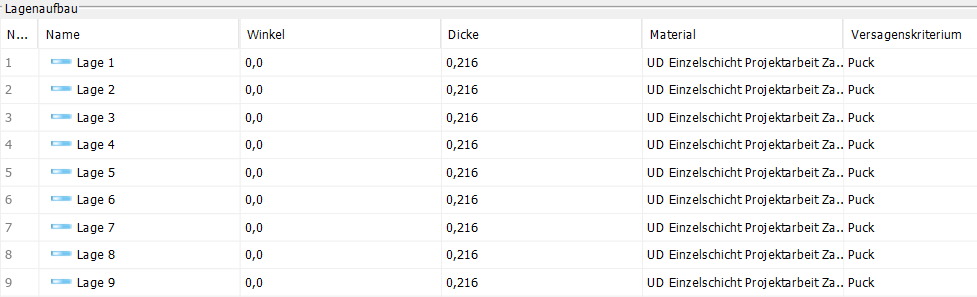
\includegraphics[width=1.0\textwidth]{Bilder/Lagenaufbau Holmgurte.png}
	\caption{Lagenaufbau Holmgurte}
	\label{fig:Lagenaufbau Holmgurte}
\end{figure}
\begin{figure}[h]
	\includegraphics[width=1.0\textwidth]{Bilder/Lagenaufbau Steg dünn.png}
	\caption{Lagenaufbau Steg Bereich $III$}
	\label{fig:Lagenaufbau Steg dünn}
\end{figure}
\begin{figure}[h]
	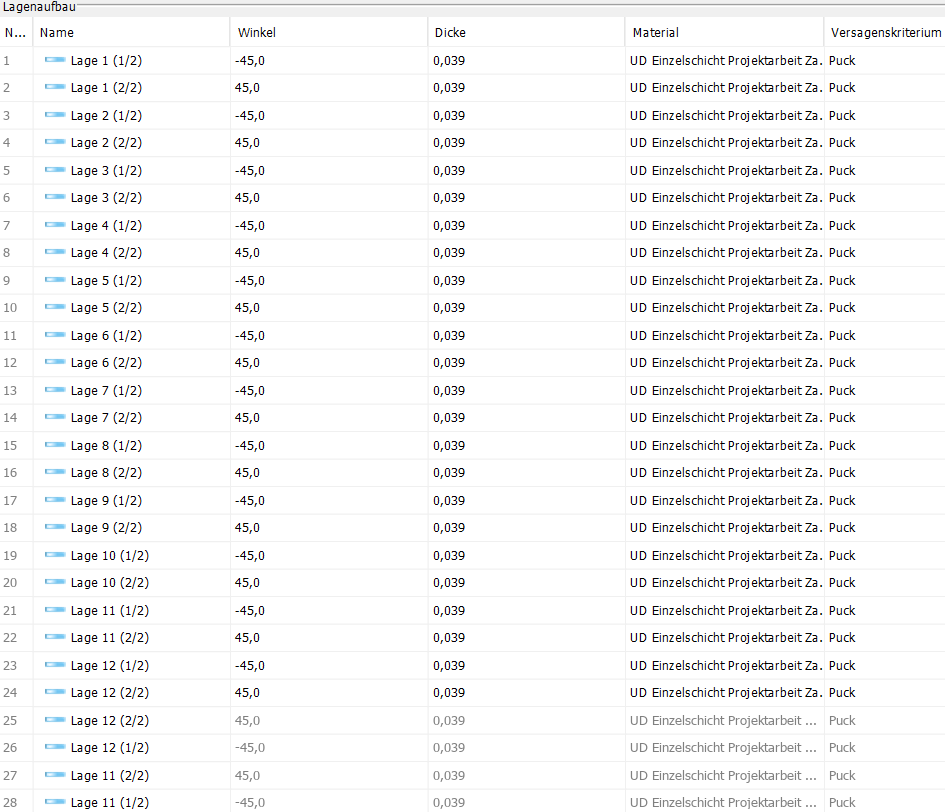
\includegraphics[width=1.0\textwidth]{Bilder/Lagenaufbau Steg dick.png}
	\caption{Lagenaufbau Steg Bereich $I$\&$II$}
	\label{fig:Lagenaufbau Steg dick}
\end{figure}
\begin{figure}[h]
	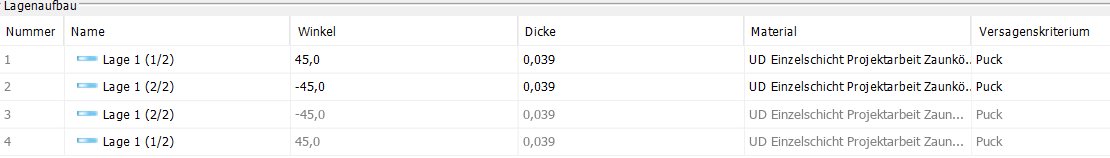
\includegraphics[width=1.0\textwidth]{Bilder/Lagenaufbau Haut.png}
	\caption{Lagenaufbau Flügelschale}
	\label{fig:Lagenaufbau Haut}
\end{figure}
\begin{figure}[h]
	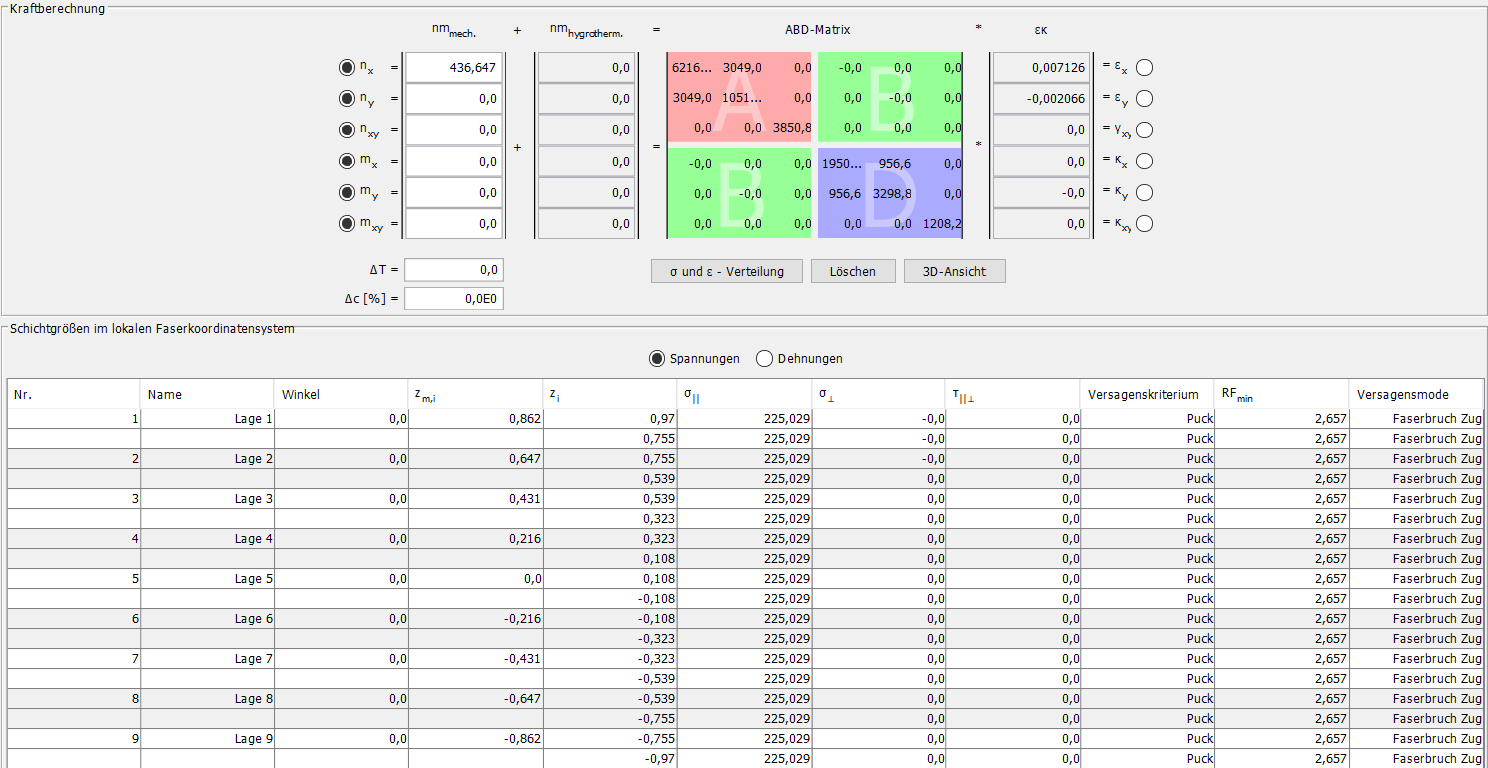
\includegraphics[width=1.0\textwidth]{Bilder/Berechnung Holmgurte.png}
	\caption{Berechnung Holmgurte}
	\label{fig:Berechnung Holmgurte}
\end{figure}
\begin{figure}[h]
	\includegraphics[width=1.0\textwidth]{Bilder/Berechnung Steg dünn.png}
	\caption{Berechnung Steg Bereich $III$}
	\label{fig:Berechnung Steg dünn}
\end{figure}
\begin{figure}[h]
	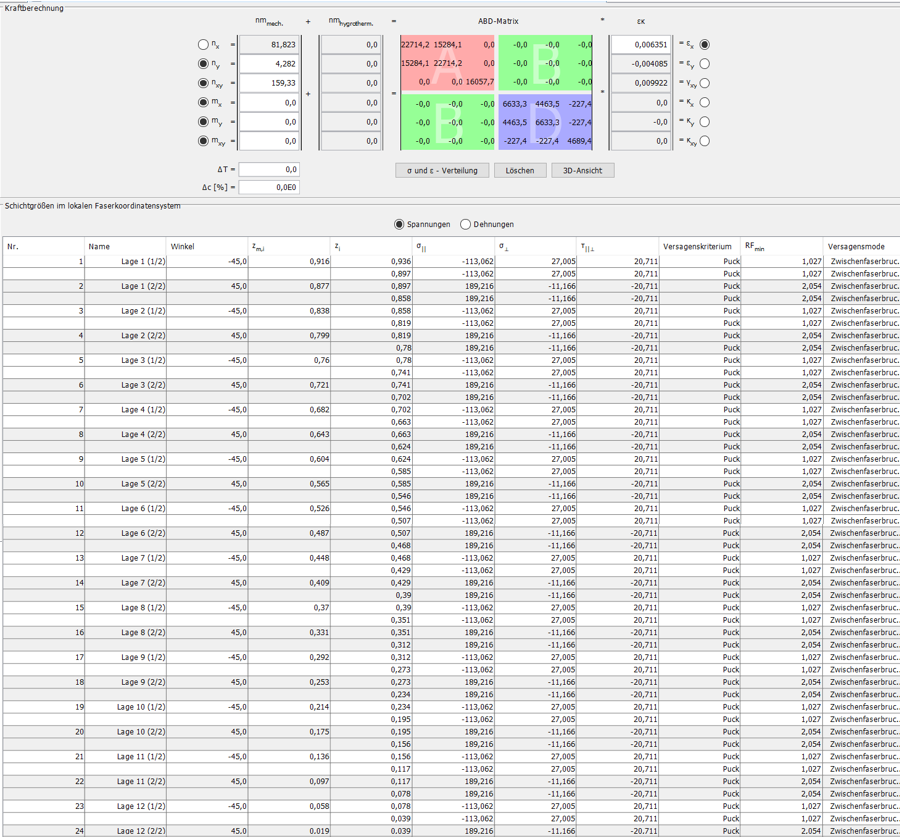
\includegraphics[width=1.0\textwidth]{Bilder/Berechnung Steg dick.png}
	\caption{Berechnung Steg Bereich $I$\&$II$}
	\label{fig:Berechnung Steg dick}
\end{figure}
\begin{figure}[h]
	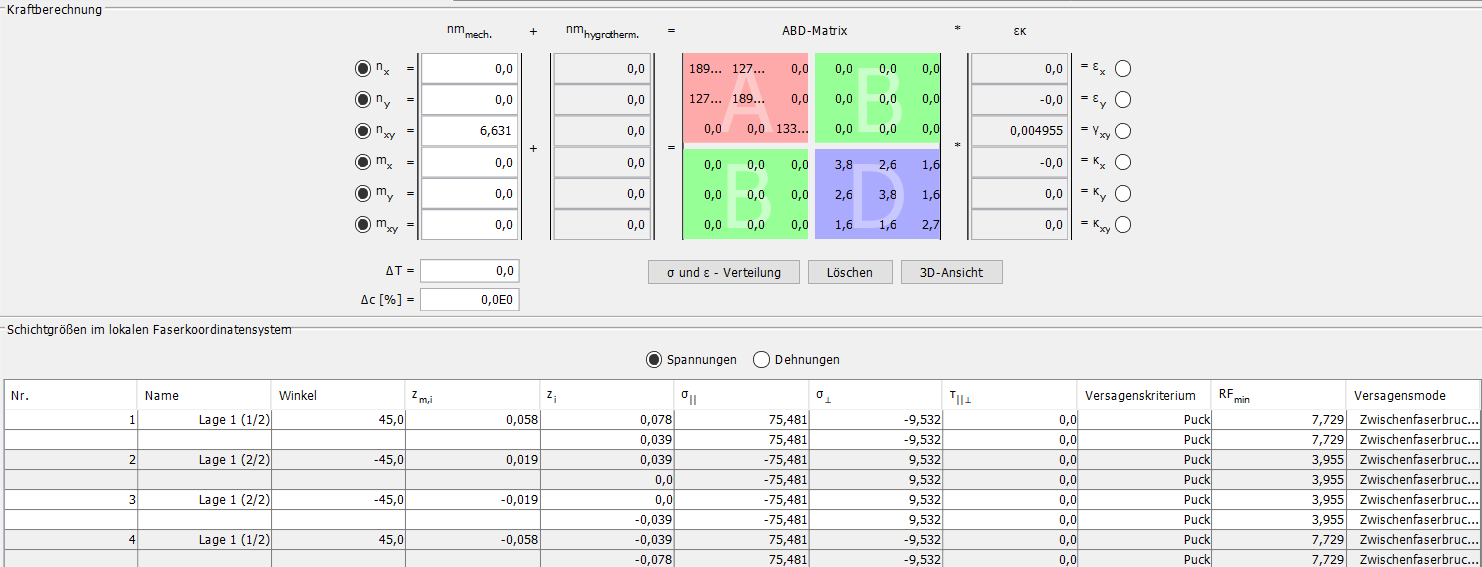
\includegraphics[width=1.0\textwidth]{Bilder/Berechnung Haut.png}
	\caption{Berechnung Flügelschale}
	\label{fig:Berechnung Haut}
\end{figure}
\begin{figure}[h]
	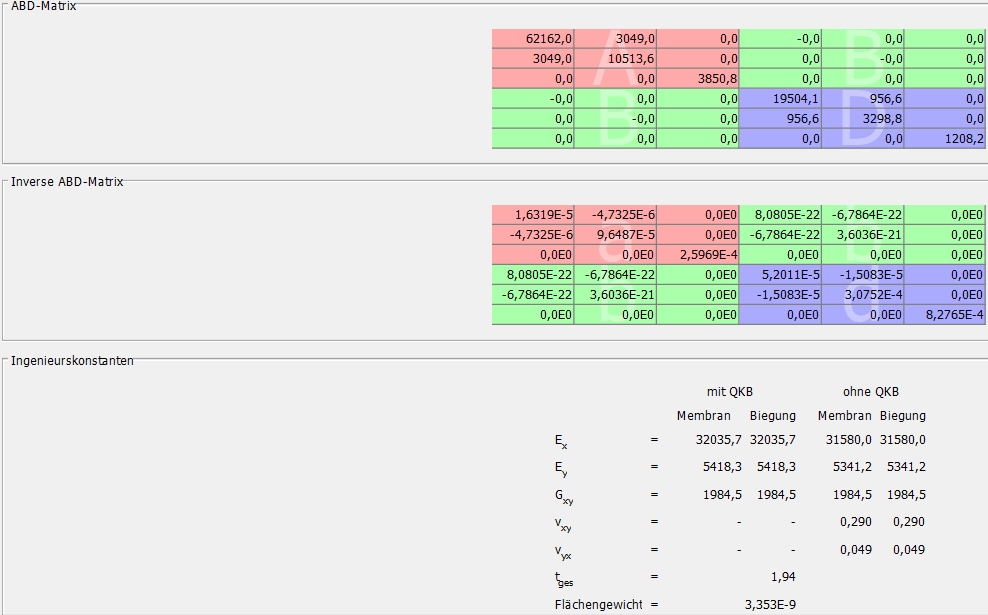
\includegraphics[width=1.0\textwidth]{Bilder/Konstanten Holmgurte.png}
	\caption{Ingenieurskonstanten Holmgurte}
	\label{fig:Ingenieurskonstanten Holmgurte}
\end{figure}
\begin{figure}[h]
	\includegraphics[width=1.0\textwidth]{Bilder/Konstanten Steg dünn.png}
	\caption{BerechnIngenieurskonstantenung Steg Bereich $III$}
	\label{fig:Ingenieurskonstanten Steg dünn}
\end{figure}
\begin{figure}[h]
	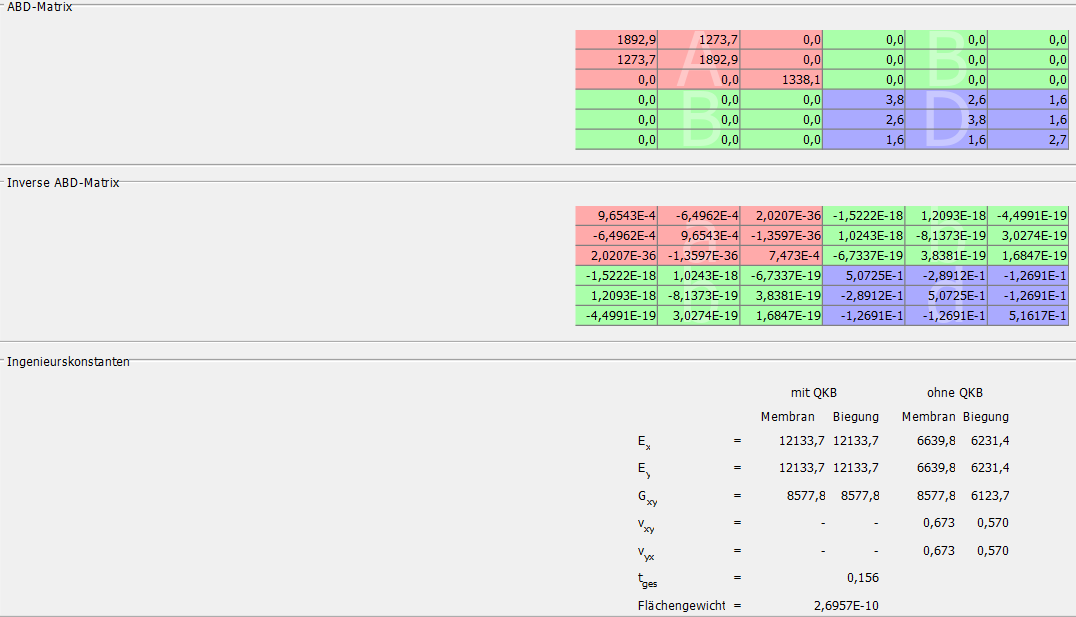
\includegraphics[width=1.0\textwidth]{Bilder/Konstanten Haut.png}
	\caption{Ingenieurskonstanten Flügelschale}
	\label{fig:Ingenieurskonstanten Haut}
\end{figure}
\begin{figure}[h]
	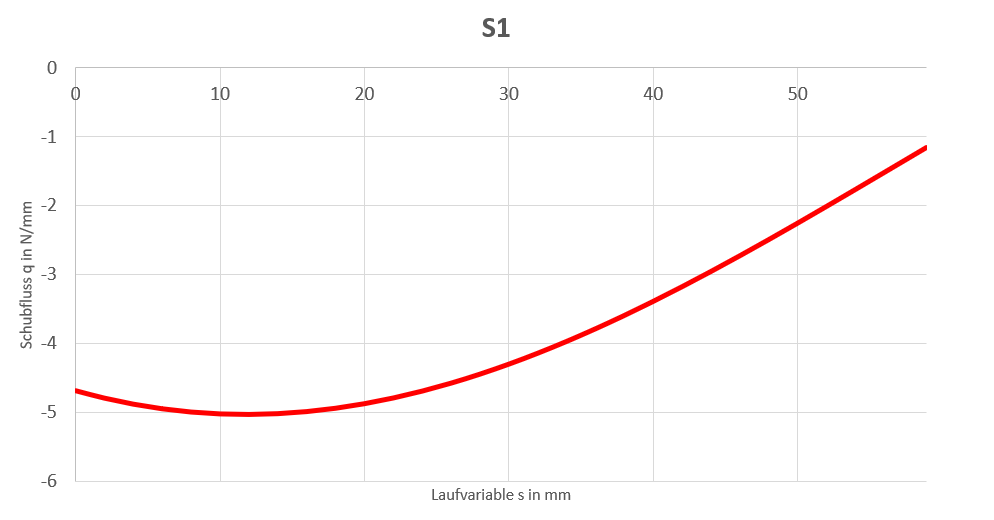
\includegraphics[width=1.0\textwidth]{Bilder/S1.png}
	\caption{Schubfluss Bereich $I$}
	\label{fig:S1}
\end{figure}
\begin{figure}[h]
	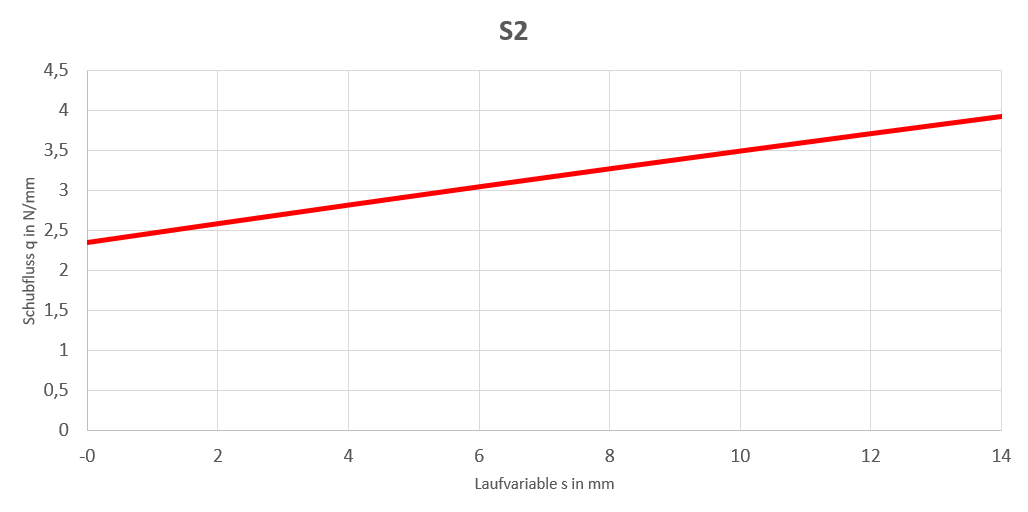
\includegraphics[width=1.0\textwidth]{Bilder/S2.png}
	\caption{Schubfluss Bereich $II$}
	\label{fig:S2}
\end{figure}
\begin{figure}[h]
	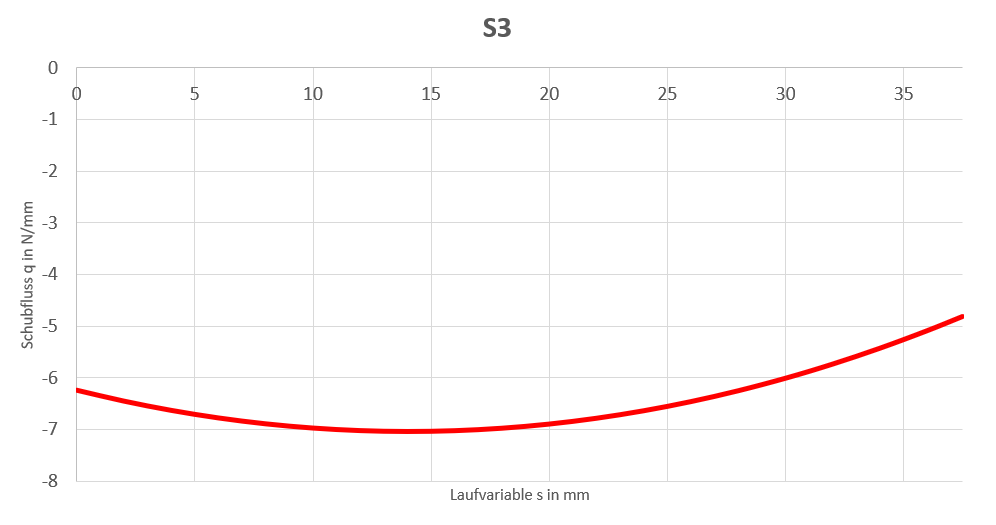
\includegraphics[width=1.0\textwidth]{Bilder/S3.png}
	\caption{Schubfluss Bereich $III$}
	\label{fig:S3}
\end{figure}
\begin{figure}[h]
	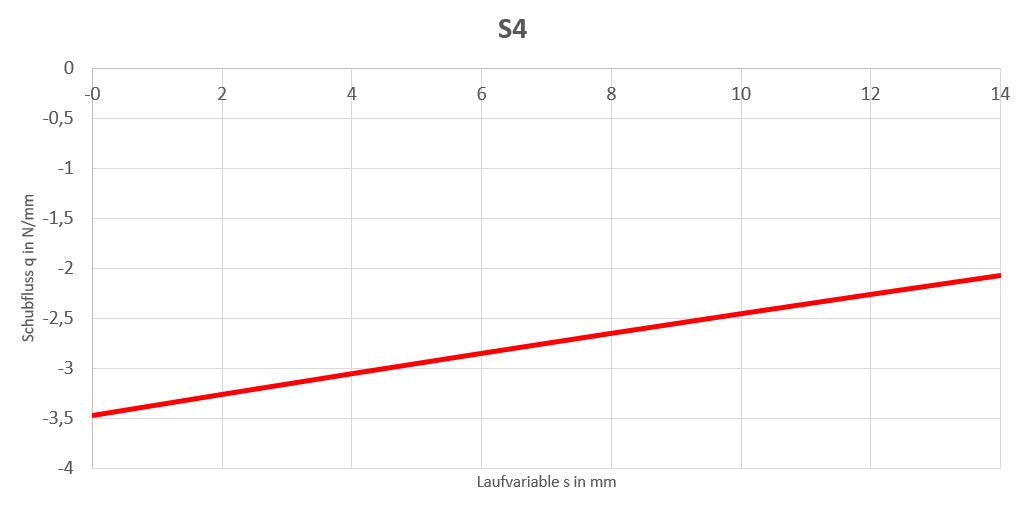
\includegraphics[width=1.0\textwidth]{Bilder/S4.png}
	\caption{Schubfluss Bereich $IV$}
	\label{fig:S4}
\end{figure}
\begin{figure}[h]
	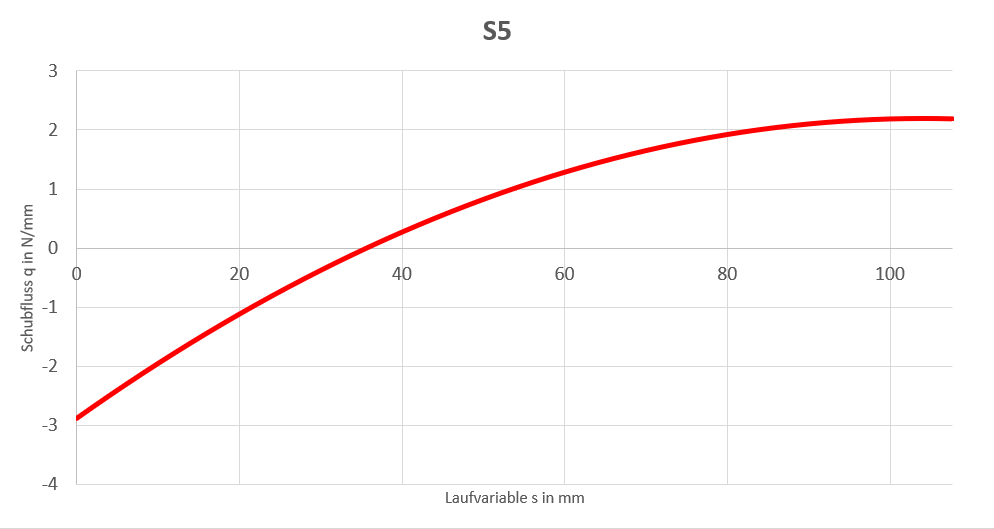
\includegraphics[width=1.0\textwidth]{Bilder/S5.png}
	\caption{Schubfluss Bereich $V$}
	\label{fig:S5}
\end{figure}
\begin{figure}[h]
	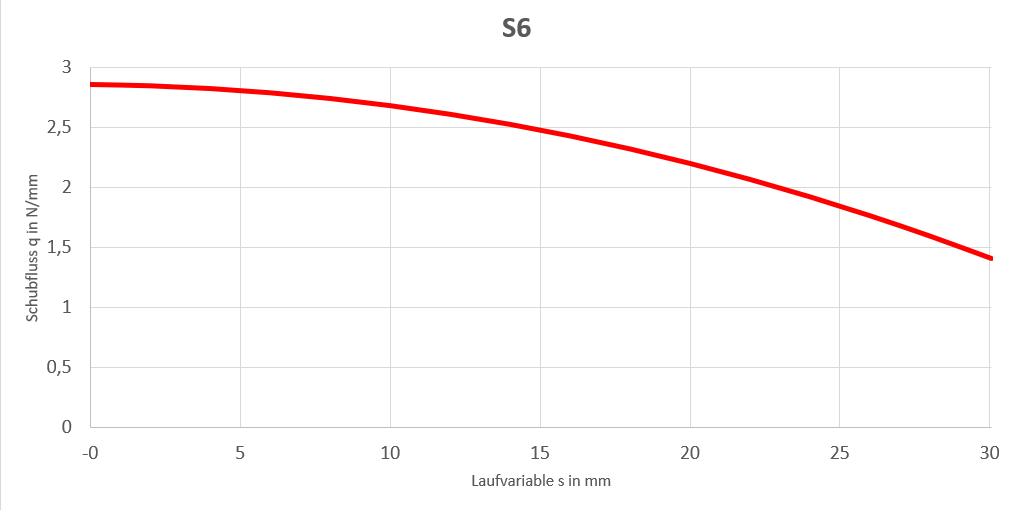
\includegraphics[width=1.0\textwidth]{Bilder/S6.png}
	\caption{Schubfluss Bereich $VI$}
	\label{fig:S6}
\end{figure}
\begin{figure}[h]
	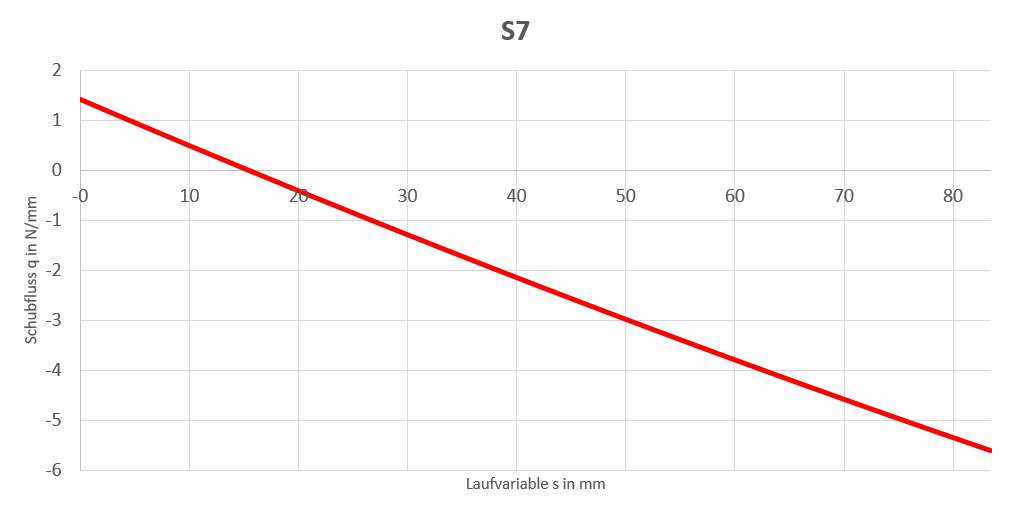
\includegraphics[width=1.0\textwidth]{Bilder/S7.png}
	\caption{Schubfluss Bereich $VII$}
	\label{fig:S7}
\end{figure}
\begin{figure}[h]
	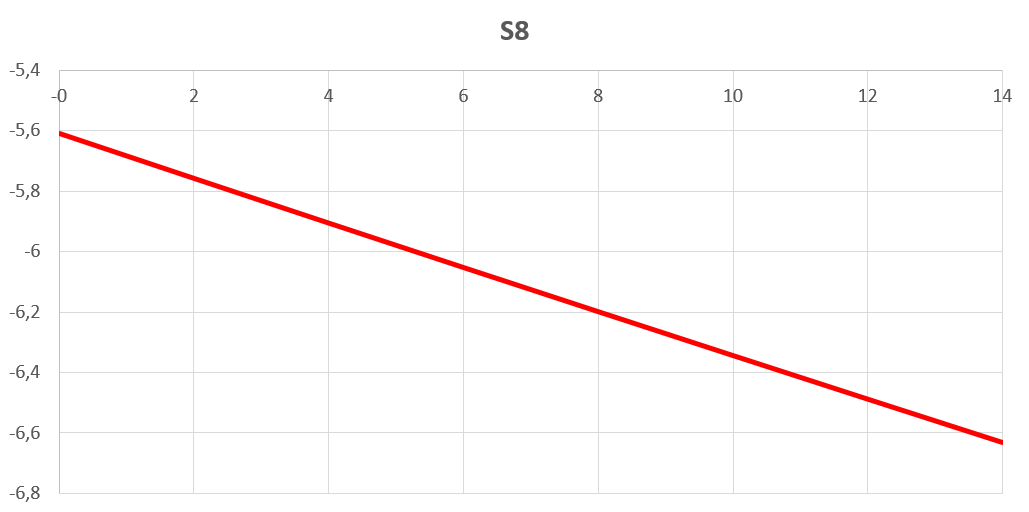
\includegraphics[width=1.0\textwidth]{Bilder/S8.png}
	\caption{Schubfluss Bereich $VIII$}
	\label{fig:S8}
\end{figure}
\begin{figure}[h]
	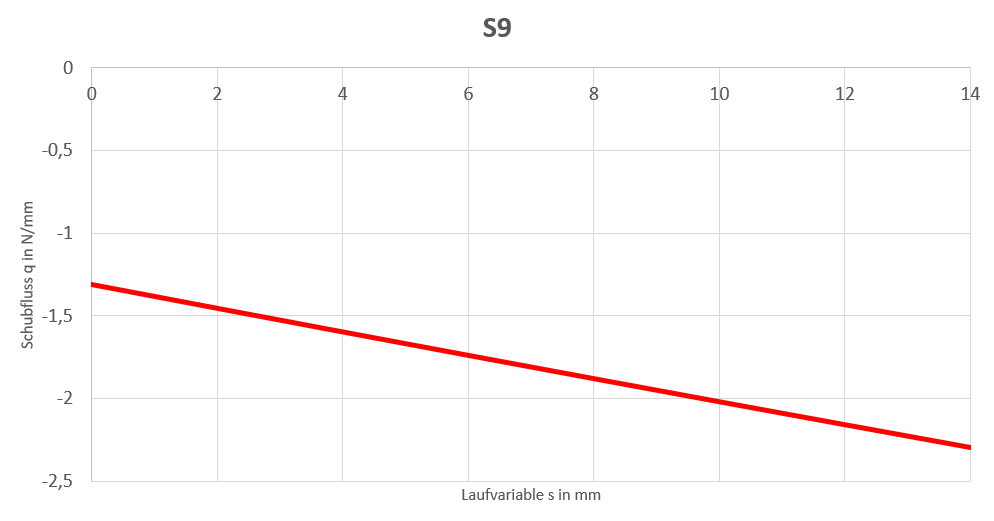
\includegraphics[width=1.0\textwidth]{Bilder/S9.png}
	\caption{Schubfluss Bereich $IX$}
	\label{fig:S9}
\end{figure}
\begin{figure}[h]
	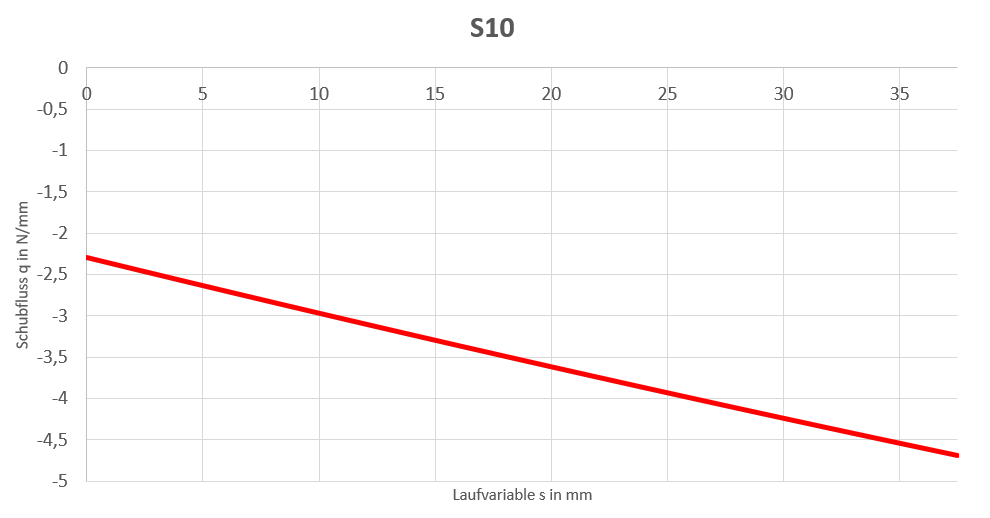
\includegraphics[width=1.0\textwidth]{Bilder/S10.png}
	\caption{Schubfluss Bereich $X$}
	\label{fig:S10}
\end{figure}



=======
Affenjunge ist
\begin{equation}
	1+1=3
\end{equation}
und 
\begin{equation}
	1*0=11
	
Je dümmer der Mensch, desto dümmer der Mensch.
Affe.
Knecht. Dirk Philipp ist ein spezieller Ingenieur, der besonders gut Schrauben auslegen kann. 


\end{equation}

Henris Test
>>>>>>> main
\end {document}